\section{Глава 1. Современные подходы к генерации ансамблей}

Текст раздела.

................................................

\begin{equation}
 \begin{aligned}
  \mathbf E^h=\pm i\mathbf H^e,\quad\mathbf H^h=\mp i\mathbf E^e. % Пример жирного шрифта
 \end{aligned}
\end{equation}

.................................................

\begin{equation}            % Пример большой формулы, где нужно переносить часть выражения на другую строчку
 \label{Eeexplicit}         % Когда нужны большие скобки, их можно открывать и закрывать с помощью \left( и \right(
 \begin{aligned}            % для случая круглых скобок. Когда надо открыть скобку на одной строке, а закрыть на другой,
  \mathbf E^e=\frac{E_0e^{-i\varphi}}{(1+2i\chi)^2}\exp\left(-\frac{\xi^2}      % надо в конце первой сроки поставить \right.,
  {1+2i\chi}\right)\left\{\left(1-\frac{\xi^2}{1+2i\chi}\right)\mathbf          % а в начале следующей - \left.
  e_x+\right.\\
  \left.+\frac{\xi^2}{1+2i\chi}(\cos2\phi\,\mathbf e_x+\sin2\phi\,\mathbf e_y)\right\}
 \end{aligned}
\end{equation}
\begin{equation}
 \label{Heexplicit}
 \begin{aligned}
  \mathbf H^e=\frac{E_0e^{-i\varphi}}{(1+2i\chi)^2}\exp\left(-\frac{\xi^2}
  {1+2i\chi}\right)\left\{\left[1-\frac{\xi^2}{1+2i\chi}-\right.\right.\\
  \left.-\frac{2\Delta^2}{1+2i\chi}\left(2-\frac{4\xi^2}
  {1+2i\chi}+\frac{\xi^4}{(1+2i\chi)^2}\right)\right]\mathbf e_y-\\
  -\frac{\xi^2}{1+2i\chi}\left[1-\frac{2\Delta^2}{1+2i\chi}\left(3-\frac{\xi^2}{1+2i\chi}\right)\right]
  (\sin2\phi\,\mathbf e_x-\cos2\phi\,\mathbf e_y)-\\
  \left.-\frac{4i\Delta\xi}{1+2i\chi}
  \left(2-\frac{\xi^2}{1+2i\chi}\right)\sin\phi\,\mathbf e_z\right\}
 \end{aligned}
\end{equation}

\begin{figure}[pH]                          % Пример рисунка, состоящего из 6 картинок
\begin{minipage}[h]{0.47\linewidth}         % Создаём "маленькие" рисунки шириной 47% от ширины страницы
\center{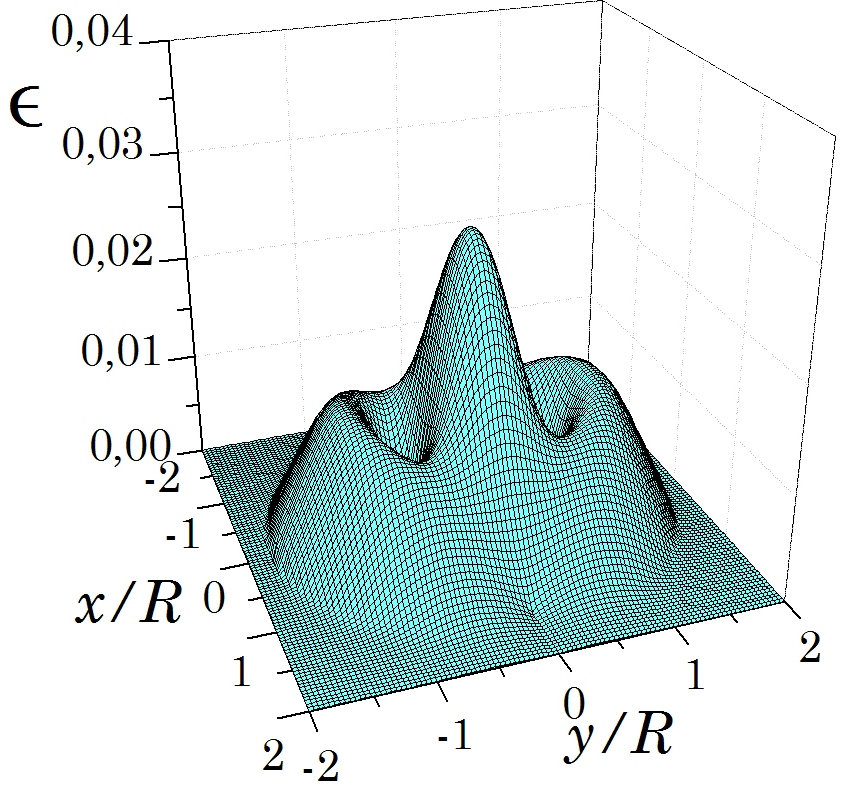
\includegraphics[width=1.0\linewidth]{images/EGraph1}} % Вставляем рисунок в полученное "окно" полностью - 100%
\end{minipage}
\hfill                                      % Следующий рисунок правее
\begin{minipage}[h]{0.47\linewidth}
\center{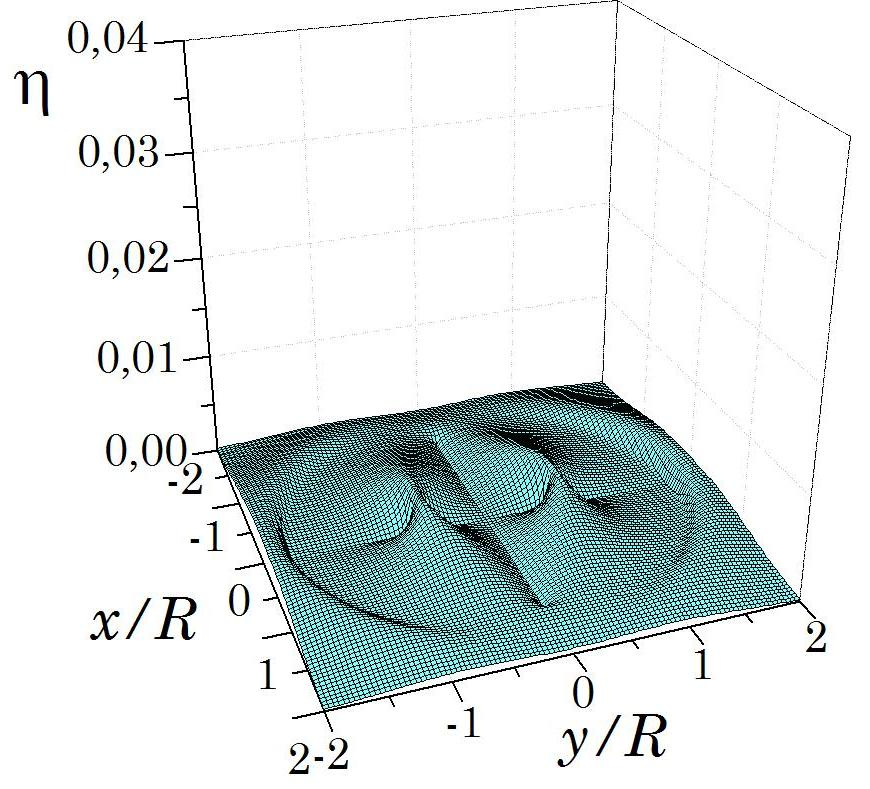
\includegraphics[width=1.0\linewidth]{images/HGraph1}}
\end{minipage}
\vfill                                      % следующий рисунок ниже - слева
\begin{minipage}[h]{0.47\linewidth}
\center{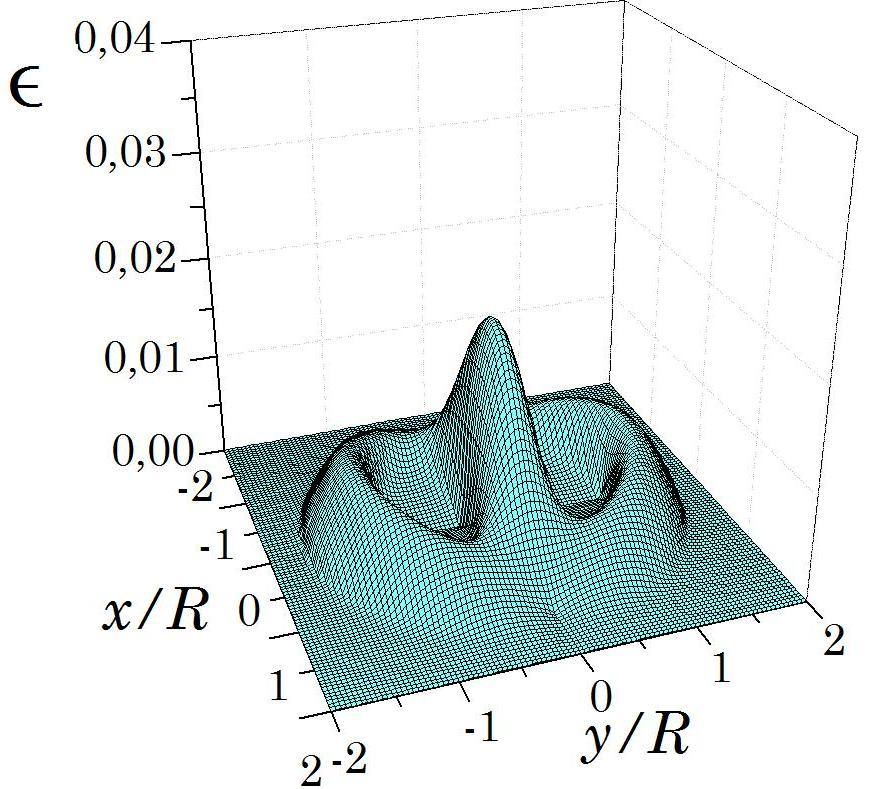
\includegraphics[width=1.0\linewidth]{images/EGraph2}}
\end{minipage}
\hfill
\begin{minipage}[h]{0.47\linewidth}
\center{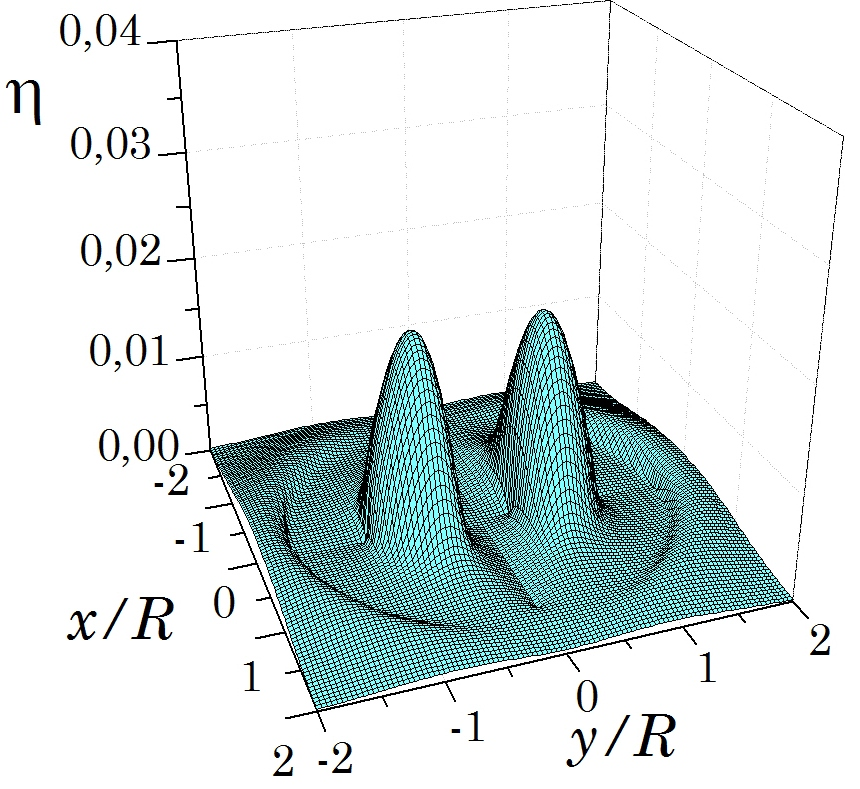
\includegraphics[width=1.0\linewidth]{images/HGraph2}}
\end{minipage}
\vfill
\begin{minipage}[h]{0.47\linewidth}
\center{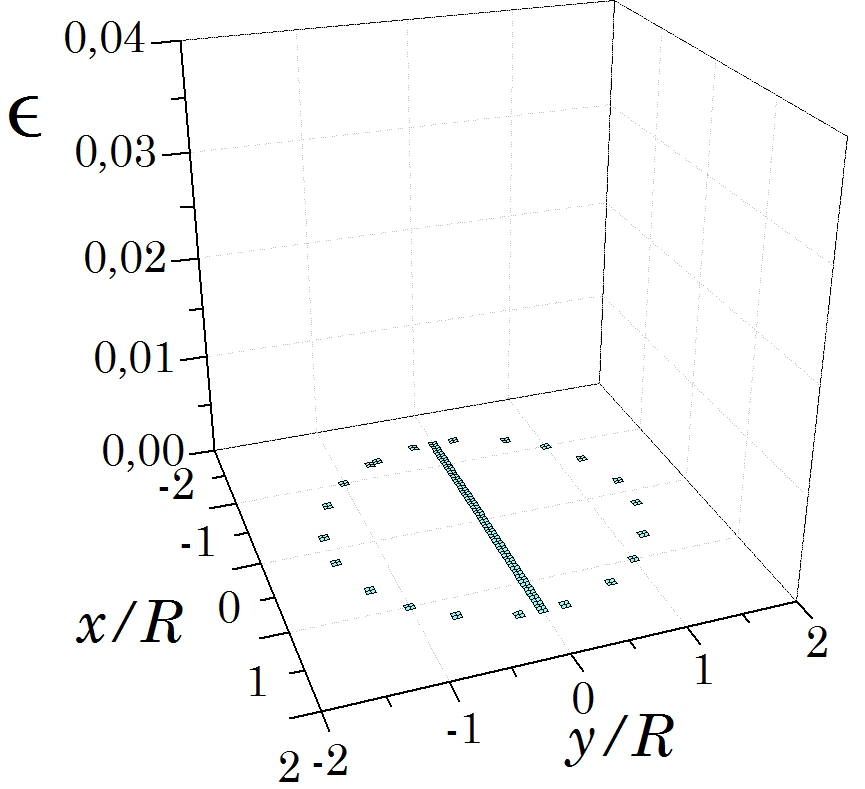
\includegraphics[width=1.0\linewidth]{images/EGraph3}}
\end{minipage}
\hfill
\begin{minipage}[h]{0.47\linewidth}
\center{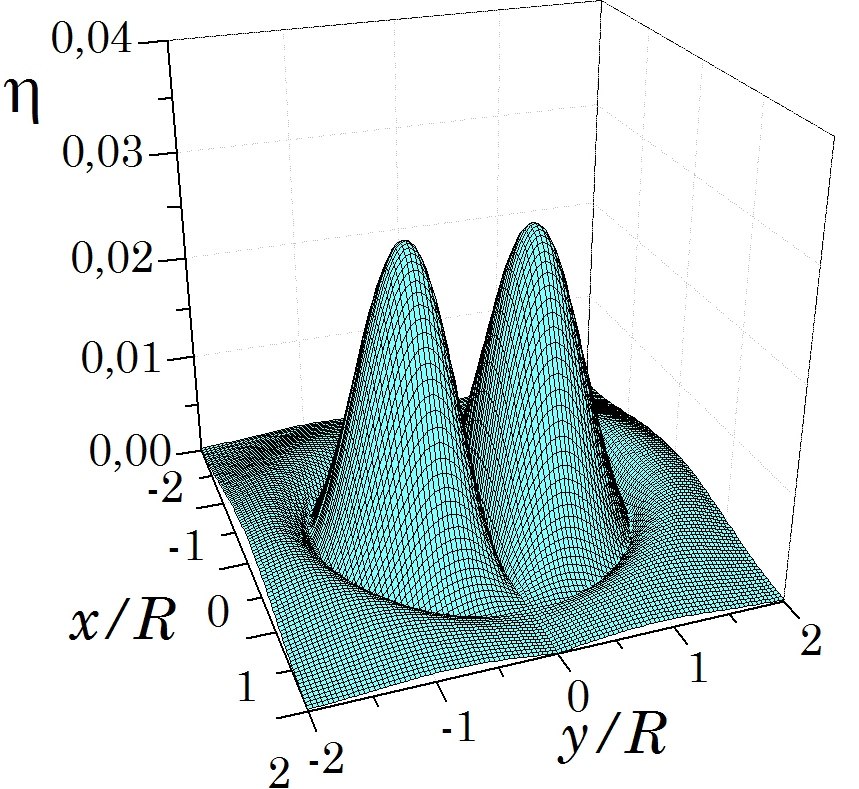
\includegraphics[width=1.0\linewidth]{images/HGraph3}}
\end{minipage}
\caption{\footnotesize Инварианты $\epsilon$ и $\eta$ для случая
одиночного линейно-поляризованного импульса $e$-типа в моменты
времени $t=0$, $t=\pi/4\omega$, $t=\pi/2\omega$. Остальные параметры
положены равными $E_0=0.1$, $z=0$, $\Delta=0.1$.} \label{EHinvs}   % Лейбл для ссылки на рисунок с помощью "рис.~\ref{EHinvs}"
\end{figure}

На рис.~\ref{EHinvs} показаны зависимости инвариантов $\epsilon$ и
$\eta$ от пространственных координат $x$ и $y$ в плоскости $z=0$ в
моменты времени $t=0$, $t=\pi/4\omega$, $t=\pi/2\omega$.
